\chapter{电场}
\section{教学要求}
这一章讲授静电学,从电菏在电场中受力和电荷在电场中具有能量两个角度出发来研究电场的基本性质。本章内容是电学的基础知识,也是学习后面各章的准备知识。

基本概念多而且抽象,是这一章的突出特点,针对这个特点,教材注意从具体情况出发引入概念,而不过于强调抽象的论证;注意加强演示实验,力求使学生获得感性知识;注意讲清楚概念的物理意义。这一章的另一个特点是许多知识要在力学知识基础上学习,教材在内容选择、确定讲述方法时注意了这个特点,希望教学中也给予注意,把新旧知识联系起来。

这一章的教材内容,是从两种电荷出发,学习电荷守恒定律和库仑定律,以此为基础,认识表征电场的力的性质和能的性质的物理量-电场强度和电势,以及它们之间的相互联系,构成较完整的静电场基础知识,作为上述知识的应用,学习了电场中的导体、带电粒子在电场中的加速和偏转、密立根实验。作为基础理论的引伸,学习了电容的概念及电容器的连接。

这一章教材可分为四个单元:第一单元包括第一节到第五节,讲述库仑定律和电场强度,第二单元包括第六节到第十节,讲述电势能、电势和电势差跟场强的关系。第三单元包括第十一节和第十二节,讲述带电粒子在电场中的运动,介绍密立根实验,第四单元包括第十三节到第十五节,讲述电容器及电容器的连接。

下面对这一章的教学内容作些具体说明。库仑定律是这一章的基础。教材详细介绍了库仑定律的实验,目的是使学生了解一些重要的物理实验方法,活跃学生的思维。教材介绍了电介质中的库仑定律,只要求学生了解什么是电介质,以及电介质中电荷间的作用力比真空中小,而不给予微观上的解释。

电场的概念,对于学生是个新概念,开始只要求大体有所了解,不要求深入地解释电场为什么是物质的一种特殊形式。电场强度和电势就是从电荷在电场中受力并具有能量这一客观事实的基础上,建立的两个重要的表征电场性质的物理概念,通过学习这两个概念以及它们的相互联系,使学生对电场的物质性有进一步的认识,由于这两个概念较抽象,又是这一章的两个教学难点,因此,在讲解电场强度之前,教材讲述了检验电荷在电场中不同位置所受的电场力的大小和方向不同的实验,使学生先对电场的强弱有所认识,便于引入电场强度的概念,对于电势的讲述,教材结合具体的电场定性地说明电势能跟电量的比值为一恒量,从而引入电势的概念,不要求作定量的论证,其目的是为了使学生容易接受一些,为了把场强和电势这两个难点分散开,在它们之间,安排讲授电场中的导体。

教材经过分析推导得出带电粒子在电场中的侧移距离和偏角公式,但不要求学生记忆这些公式,应该注意培养学生运用物理规律对具体问题进行具体分析的能力。讲述这一内容时,还要综合运用力学和电学知识,有利于发展学生综合运用知识的能力,教学中要予以重视。

密立根实验是物理学的经典实验之一,教材介绍了这个实验的基本思路,限于学生知识基础,不要求进一步讲解密立根是如何测定油滴半径的,不要求讲解密立根实际所做的实验。这个实验只讲给学生,不要求实际去做。

电容的概念比较抽象。教材讲述了平行板电容器的电容,并给出了公式,其目的在于让学生领会电容是由电容器本身的因素决定的,不要求用公式进行定量计算。

教材介绍了静电的应用及其危害,是为了加强理论知识与实际的联系,以利于扩展学生眼界。

这一章的教学要求是:
\begin{enumerate}
\item 了解电荷守恒定律,掌握库仑定律,能够计算点电荷间的相互作用。
\item 了解电场的概念,理解电场强度和电力线,掌握电场强度的公式和单位,了解匀强电场的特点。
\item 理解导体处于静电平衡时的特点。
\item 理解电势能、电势、电势差的物理意义,了解等势面.掌握匀强电场中场强和电势差的关系。
\item 掌握带电粒子在电场中的运动规律,能够分析解决加速和偏转方面的问题。
\item 了解密立根实验的简单原理和测定基本电荷的意义.
\item 理解电容器的电容概念、掌握电容器串联和并联的公式。
\item 了解静电的应用.
\end{enumerate}

\section{教学建议}
\subsection{第一单元}
\subsubsection{两种电荷}

教学中首先要利用实验演示电荷的种类、电荷的相互作用、电荷的相互增强和减弱、抵消等现象。比如,用一绝缘线悬挂一导体球,使其带上某种电荷。用毛皮摩擦后的橡胶棒接近它时,相互排斥;用丝绸摩擦后的玻璃棒接近它时,相互吸引。这说明橡胶棒和玻璃棒上带两种不同的电荷.再通过讨论问题:
\begin{enumerate}
    \item 什么叫物体带电?电荷有哪两种?它们之间有怎样的相互作用?
    \item 什么叫电荷的相互增强和中和?
    \item 摩擦起电的过程是怎样的?
\end{enumerate}
使学生回顾和复习初中的静电知识。

然后,结合演示实验讲解什么是静电感应和感应起电,这里只说清楚现象,理论解释留在电场中的导体一节讲述。至此,可以归纳已学过的起电的各种方法(接触起电、摩擦起电和感应起电)的特点,使之对起电过程,即使物体中电荷分离的过程有较深的理解。

\subsubsection{电荷守恒定律}

充分运用前面演示实验的事例:课本
图6.1所示的电荷相互增强和中和的现象,摩擦起电的过程,课本图6.2所示的静电感应现象的分析;说明以下问题:电荷的中和是否正、负电荷都消失了?物体呈中性,是否说明物体中没有电荷?感应起电中,是否导体两端新产生了正、负电荷?从而得出荷守恒定律的内容,强调在电荷的分离和转移的过程中总量保持不变。

\subsubsection{库仑定律}

从初中对电荷间相互作用的认识过渡到对相互作用力的定量研究,首先就要弄清楚电荷间相互作用力的大小和方向。库仑定律就是反映这种关系的物理规律,是电学的基础规律。

点电荷的概念,可以从质点的概念出发来理解。指出这是一个理想化模型,明确在哪种实际情况下,可以把带电体科学地抽象为点电荷,强调研究点电荷间的相互作用,是库仑定律成立的前提条件。

得出库仑定律,是以库仑扭秤实验为基础的,通过教学,不仅可以了解库仑定律的建立过程,而且能学到一些物理实验的方法,这个实验不要求实际去做,但应运用模型或挂图,以增强教学的直观性。同时,要引导学生联想卡文迪许实验验证万有引力定律的过程,以帮助学生了解库仑扭秤实验装置和原理。教学中可采用讲解或自学讨论的方法,如果用后一种方法,可提出以下问题:库仑是用什么办法测算出点电荷间的作用力的?当时还没有电量的单位,库仑是怎样解决作用力与电量的关系的?让学生带着问题阅读教材,展开讨论,明确库仑扭秤实验的过程。当然,要指出两个金属球必须是大小相同的,但不必说明理由。

对库仑定律的内容,要把文字表述和数学表达式结合起来理解,还要把库仑定律和万有引力定律作对比,以利于记忆和应用,要再次强调定律成立的条件是点电荷,指出它的适用范围可以推广到静止的电荷与运动电荷之间的相互作用(例如原子核对运动电子的作用);运动电荷间的相互作用则不适用了。

电介质中的库仑定律,可以用两个相互作用的带电小球间插入一电介质(如塑料板)后,其作用力减小的现象推理得出:如果这电介质充满空间,两个带电小球的相互作用力比在真空中的要小,这样对公式$F=kQ_1Q_2/\varepsilon r^2$的理解就会容易一些,对电介质的意义和介电常数,只作介绍,不作深入探讨。

在应用定律进行运算时,电量要用绝对值代入,力的方向由是引力或斥力具体确定,公式中各物理量的单位都统一使用国际单位制的单位。

在解决多个点电荷间作用问题时,要注意每两个点电荷间就有一对库仑力,它们遵从牛顿第三定律。

在解决综合力学问题时,带电体不仅受到库仑力,还可能受到万有引力(重力)、弹力、摩擦力的作用。教材的例题计算结果说明,在研究微观粒子的相互作用时,库仑力比万有引力大得多,因而万有引力可以忽略;但在其他带电体的平衡或运动的问题中,是否可以忽略万有引力(重力),应视具体情况而定。

以上各点,应结合例题、习题的教学,尽可能启发学生自行得出,使之易于理解、记忆和应用。

\subsubsection{电场和电场强度}

电场是学生新接触的抽象概念,教
学时要加强直观性,做好课本图6.4甲的演示实验,可以采用讲解法,与磁极间的相互作用比较,由学生已有的磁场概念形成对电场的认识,再结合对电磁场、电磁波及其应用于实际的广播、电视的介绍,帮助学生理解电场是一种特殊的物质。并指出电场的物质性的表现之一,就是它对其中的电荷具有力的作用。

关于电场强度的引入,首先要讲清检验电荷的意义。为了感知电场的存在及其性质,要用检验电荷进行探测,只有点电荷,由它来确定电场中某点的位置才有确切的意义;只有带电量很小,它自身的电场对源电荷电场的影响才能忽略。然后,做好课本图6.4甲所示的实验,定性地说明检验电荷在电场中的不同位置,所受电场力大小不同,进而说明电场各点的强弱不同,为此引入电场强度这个物理量。

讲解电场强度的定义时,可提出“能否用电荷所受电场力的大小表示电场的强弱”这一问题来思考,引导学生回忆密度的概念:对某种物质,体积大的质量大,用单位体积的质量、即密度来表示物质的这种特性;在电场中某点,电荷的电量大受到的电场力就大,用单位电量的电荷受到的电场力、即电场力与电量的比值,表示电场的力的性质——电场的强弱,再利用课本图6.4乙,以点电荷电场中的$A$点为例,分析电场力随电量的变大而增大,概括出电场力与电量的比值相同;对不同的点则比值不同,由此抽象出这个比值与检验电荷的电量无关,表示电场本身的性质:在比值大的点电场强,在比值小的点电场弱。并把点电荷电场的定义推广到任何电场。

场强的方向,可以在课本图6.4乙的基础上来说明,以$+Q$为圆心、以$r_1$为半径作圆,在圆上取任一点$D$, 说明$A$、$D$两点场强的大小相等,同一电荷分别在这两点所受的电场力力大小相等,但力的方向是不同的。从而说明场强是有方向的,是矢量,然后再进一步指出,场强的方向是怎样规定的。由于场强是矢量,对几个电场的叠加,其合场强要用平行四边形法则进行矢量运算;对此,只要求简单介绍,不要求定量计算。

可以把电场强度与电荷所受的电场力,从意义、公式、方向、单位等方面用列表的形式,加以比较,加深对场强的理解。还应该通过解答习题,帮助学生认识公式$E=F/q$与公式$E=kQ/r^2$和$E=kQ/\varepsilon r^2$的区别和联系。

\subsubsection{电力线}

先通过讲解,明确引入电力线可以形象地表示电场分布。再演示悬浮在蓖麻油中的木屑在各种电场(正、负点电荷的电场,两个等量异种电荷和等量同种电荷的电场)中排成一系列直线或曲线的情况。再说明电力线是人为设想的,不是真实存在的。最后讲述电力线的定义,说明线上各点的切线方向,与该点的场强方向一致。

匀强电场是最简单而又很重要的电场,要在演示木屑微粒在带正,负异种电荷的平行板间的分布形状的基础上,讲清什么是匀强电场?它的场强的特点和电力线分布的特点是什么?实际的匀强电场有哪些?

\subsubsection{电场中的导体}

教材先用分析推理的方法,讲述导体在电场中的一些基本性质,然后用实验验证,希望能发展学生的推理能力。为了激发兴趣、设置悬念,加强直观,可以先演示带电小球在电场中受力、小球罩上金属空腔后又不受电场力的现象。再提出问题:电场中的金属空腔为什么能起这样的作用:把研究金属空腔,转变为研究电场中的导体。

引导学生复习金属导体的组成和导电的微观机制,有层次地讲解:
\begin{enumerate}
\item 导体在电场$E$中,内部的自由电子受电场力作用作逆电场方向的定向移动,导致垂直于场强方向的两端面出现等量异种电荷;
\item 同时,这种电荷将在导体内形成与外电场$E$方向相反的附加电场$E'$;
\item 在$E'<E$时,自由电子的定向移动按原方向继续进行,两端面积累的电荷增多,附加电场$E'$增强;
\item 当$E'=E$时,导体内部自由电子的宏观定向移动停止,处于动态平衡状态,两端面积累的电荷稳定;由于$E$与$E'$叠加的结果,导体内的合场强为零,因而没有电力线分布。
\end{enumerate}
在以上的讲解的基础上,说明静电平衡状态的意义,以及在这种状态下场强的特点。

导体在静电平衡时其表面上任一点的场强方向与导体表面垂直和电荷只能分布在导体表面,教材都是用反证法来说明的,学生不易理解;教师既要讲清知识,又要讲清思路。之后,再用演示实验验证。

\subsection{第二单元}
\subsubsection{电势能}

教材是直接与重力势能类比,引出电势能概念的,不要求论证移动电荷做功与路径无关。具体地以异种的场源电荷和检验电荷为例,把场源电荷与地球、检验电荷与物体类比,从重力势能和重力做功跟重力势能变化的关系,来认识电势能和电场力做功跟电势能变化的关系。教学中,可以在复习重力势能、正功、负功等知识的基础上,引导学生列表对比进行讨论。应指出,由于电场力可以是引力也可以是斥力,因此电场力做功的问题要复杂一些。

教材中结合正、负电荷的电场来讲解电势能,对正电荷在电场中不同位置时电势能的大小、数值、正负分别作了说明,以期学生对电势能的认识更加具体,讨论正电荷$q$在$+Q$和$-Q$的电场中不同点电势能的大小时,可按以下顺序进行:
\begin{enumerate}
\item 确定$q$所受电场力的方向和它在电场中两点间的位移方向;    \item 根据两者的方向关系,判定电场力做正功还是负功;    \item 由电场力做功跟电势能变化的关系,判定电荷$q$在电场中两点电势能的大小;    \item 得出结论:在$+Q$的电场中,电荷$q$离$+Q$越近,电势能越大;在$-Q$的电场中,电荷$q$离$-Q$越近,电势能越小。在教学中,第一种情形由教师示范讲解,第二种情形可由学生自行推出结果,以利培养学生的推理能力。
\end{enumerate}

在讨论电势能的数值时,可先复习重力势能的数值是怎样确定的,再与重力势能类比,以正电荷$q$在$+Q$和$-Q$点电荷的电场中为例,讲请确定电势能数值的过程。要先确定电势能为零的位置,一般取电荷$q$在无穷远处的电势能为零,把电荷$q$从电场中某点移到零电势能处电场力做功的大小,即为电荷$q$在电场中某点电势能的数值。

在讨论电势能的正负时,要先复习重力势能正负的意义。然后,仍以$+Q$和$-Q$点电荷的电场为例,讲清在$+Q$的电场中,将正电荷$q$从任何一点移向无穷远(零电势能)处,电场力做正功,电势能减小至零;因而正电荷$q$在$+Q$电场中任
何一点的电势能都是正值。同理,可以说明正电荷q在$-Q$的电场中任一点的电势能都是负值。需要强调,这结论是检验电荷为正的条件下得出的;若检验电荷为负电荷,则结论不同。

\subsubsection{电势}

在引入电势之前,可复习场强的引入过程,说明在电场中某点,随着检验电荷电量的增大,所受电场力成正比地增大,但电场力与电量的比值是确定的,这就是该点的场强。它与检验电荷的电量无关,是表示电场力的性质的物理量。与场强的引入过程类比,结合具体的电场定性地说明:在电场中某点,检验电荷的电势能随电量的增大而成正比地增大,但电势能与电量的比值是确定的,它就是表示电场的能的性质的物理量,从而引入电势。电势的高低也与检验电荷的电量无关,由电场本身的性质决定。

与电势能对应,讲明零电势位置的确定;以及它确定后,电场中各点电势的大小才有确定的数值,电势的正负才有确切的意义。再应用上述认识,说明点电荷$+Q$和$-Q$的电场中各点电势的高低,从而得出结论:在$+Q$的电场中,电势都为正值,离$+Q$越近电势越高;在$-Q$的电场中,电势都为负值,离$-Q$越近电势越低。

根据电力线的方向可以判定电场中各点电势的高低,为帮助学生理解,可先列举电荷在如课本图6.16的电场中的各点间移动时,根据电场力做功的正负,判定电势能的变化,进而判定电势的高低,再考察电力线的方向与这些点的电势高低的联系。最后概括得出:顺着电力线方向,电势越来越低。

要及时帮助学生小结已学过的知识,可以把电场强度与
电势、电势与电势能,分别列出表格,从意义、公式、方向性、单位等方面进行比较,巩固掌握这些概念,也发展了分析、比较的思维能力。

\subsubsection{等势面}

首先,要明确什么是等势面?可以运用地图上等高线作比喻,以点电荷的电场和匀强电场为例,配合模型教具,讲清等势面的意义。

电力线与等势面的关系,可先用反证法得出:等势面一定跟电力线垂直;再在复习电力线方向与电势高低的关系的基础上得出:电力线是由电势较高的等势面指向电势较低的等势面。注意运用这些知识,分析具体的各种电场中电力线与等势面的关系,了解和想象这些电场的等势面的形状。

在讲解带电导体(课本图6.22)周围的电场中等势面的分布时,要讲清“处于静电平衡状态的导体是等势体,其表面是等势面”,使学生对处于静电平衡状态的导体的力的性质(场强)和能的性质(电势)的特点,有全面的认识。

\subsubsection{电势差}

引入电势差时,除用地理位置的高度差不变
来比喻外,还可以列举数据阐述或指导学生运算,说明在匀强电场中,选定不同的零电势位置,其中任意两点的电势之差保持不变,进而指出电势差的应用比电势更普遍,它的物理意义和公式也就顺势得出了。讨论电势差在$U_A>U_B$和$U_A<U_B$的两种表示式,是为了表明:两点间的电势差要取绝对值,又要明确哪点的电势高。还要用公式说明,电场中某点的电势,就是该点相对于零电势位置的电势差。

用电势差来计算电场力做功时,公式中各物理量取绝对值,电场力做功的正负要根据电荷移动方向与所受电场力方
向的具体情况来判定。

\subsubsection{电势差和场强的关系}

讨论电势差和场强的方向的关系时,为了便于学生接受,可以举例说明,自山顶上从坡度不同的两个方向下到同一水平面,坡度陡的方向,单位长度的水平距离上高度下降大,即高度下降得快,再结合课本图6.24的匀强电场讲解,$AB$、$AC$、$AD$三个方向,电势下降的差值都相同;$AB$的距离最小,单位长度上电势降落最大,即电势降落最快;而$AB$的方向就是场强的方向,因而得出:场强的方向是指向电势降低最快的方向。

在得出电势差和场强在数值上的关系式$E=U/d$后,要强调理解公式的意义和适用条件,$d$是两点间在场强方向上的距离,$U$是所对应的两点间的电势差;它只对匀强电场才适用。

\subsection{第三单元}
本单元的内容,是以带电粒子在电场中的运动和密立根实验为例,应用电场和力学的知识解决综合性问题。由于这部分内容主要是已学知识的运用,可较多地放手让学生自行探讨、研究,以利于对电场知识的深人理解和巩固,培养学生分析和解决问题的能力。

\subsubsection{带电粒子的加速和偏转}

为了增强学生的感性认识,可以演示阴极射线管,说明热电子在加速电场作用下,形成电子束;演示阴极射线管或其他带电粒子在电场中偏转的现象。要复习力学中匀加速直线运动和平抛运动的有关知识,以便
为学生学习这一部分知识作好准备。

结合课本图6.27和图6.28, 可引导学生应用已学的电学和力学知识自己去探讨研究。对带正电粒子的加速,要求学生分别用牛顿运动定律和动能定理,推导出带电粒子达到负极板时的速度$v=\sqrt{2qU/m}$, 对带电粒子的偏转,要求学生对照物体在重力场中的平抛运动,从受力、加速度、飞行时间、侧移距离、末速度$v$与初速度$v_0$的夹角$\phi$, 逐步推导出侧位移$y$和夹角$\phi$的表达式,并讨论决定$\phi$的因素。

还可以深入讨论下述一些问题。比如,在带正电粒子加速的现象中,可以提出:
\begin{enumerate}
\item 若粒子以速率$v_0$从正极板小孔沿场强方向进入电场,则从负极板小孔穿出时的速率$v$有多大?
\item 若粒以初速度$v_0$从负极板小孔沿场强方向进入电场,粒子作什么运动?为什么?
\item 如果不是匀强电场,能否用匀变速动公式求出粒子到达负极板的速率?为什么?应该怎么办?
\end{enumerate}


要概括讲解分析和解决问题的思路:对带电粒子进行受力分析(包括电场力),明确粒子的运动状态及过程,运用相应的力学规律列式求解。

\subsubsection{密立根实验}

这个实验是较精确地测定基本电荷数值的重要物理实验。应向学生讲解基本电荷的概念,简述电子发现的过程及有关测定电子电荷量的实验。这个实验只要求学生懂得道理和方法,不要求实际去做。

要先介绍实验的设想:如果电子的电量是基本电荷,那么,测出若干个带电微粒的电量,如果这些电量都是某一电量的整数倍,这个电量,即为基本电荷。接着,讨论下面的问题:
\begin{enumerate}
\item 实验研究中用的是什么微粒1怎样使它带电的?
\item 根据什么原理、使用怎样的装置、采取什么方法测得带电微粒的电量?
\end{enumerate}
通过讨论,明确测微粒电量的原理和方法。对计算式$q=mgh/U$中,油滴质量$m$的计算,应作简要的说明。在对数千个油滴电量的实验数据进行分析研究后,才得出基本电荷的数值$e$.

在上述讨论、说明的基础上,讲述实验原理。实验是根据带电油滴在电场中平衡时,所受合力为零来计算油滴的荷电量的,进而应用数学知识进行分析研究,求得基本电荷数值的。带电微粒在电场中平衡时,受力分析一般要考虑重力。

\subsection{第四单元}
\subsubsection{电容}

可以从电视机、电子仪器中广泛使用电容器,
引入对电容器的学习,让学生观察废旧的电容器的外形及电极,再把它拆开,看两个极板(金属箔)和中间的电介质,了解电容器是由两个彼此绝缘又相互靠近的导体构成的。再演示电容器充电和放电的现象,配合讲解,说明充电后,电容器两极板带上等量异种电荷,电容器的功能就是能够容纳(储存)电荷。要强调指出:电容器所带的电量,是指一个极板带电量的绝对值。

不同电容器容纳电荷的本领是不相同的,可从怎样表征这一性质,过渡到电容概念的教学,电容器这个概念比较抽象,教材把它与容器的容量作了对比,既然是对比,就不可能完全相同,达到有助于理解电容的目的就可以了。

还可以用场强、电势等用比值定义的物理量作类比,加深对电容概念的理解。

\subsubsection{平行板电容器}

这里讨论的是决定它的电容大小的因素及相互关系,使之对电容的物理意义有深入的认识。讲清这一问题的前提是做好教材要求的演示实验,在介绍实验装置时,应讲清静电计指针张角的大小为什么能够表示电容器两极板间电压的大小。在进行操作前,可以先把观察现象的记录表格板画出来,使学生观察有目标,并在演示中及时记载结果。根据实验结果,概括出平行板电容器电容公式$C=\dfrac{\varepsilon S}{4\pi kd}$, 可以用已学过的知识,对公式作定性说明,还要指出,这个公式与电容定义式的区别和联系,以及它只适用于平行板电容器这一条件。

要通过练习或例题说明,使用公式$C=Q/U$讨论平行板电容器的有关问题时要注意:
\begin{enumerate}
    \item 若电容器两极板与电源相连接,则极板间的电压不变;
    \item 若电容器极板与电源断开,则极板的荷电量不变。
\end{enumerate}



\subsubsection{电容器的连接}

讲述电容器的串联和并联,可从连接方法、电量关系、电压关系和电容计算等方面通过讲解或指导学生推证,用列表的方法加以比较。

根据静电感应的原理,讲清串联电容器中的每个电容器极板带电量相等,且等于电容器组的总电量,根据电荷守恒定律,讲清并联电容器组的总电量等于每个电容器所带电量之和。根据电容器各级板的电势关系,分析得出:串联电容器
的总电压等于各个电容器极板电压之和;并联电容器中各个电容器极板间的电压相等,且等于总电压。上述结果,还可以用电压表对实际电路中各个电压的测定数据进行验证。

两种连接法的电容的计算,或教师讲解、或指导学生用公式推导,得出
\[\frac{1}{C_{\text{串}}}=\frac{1}{C_1}+\frac{1}{C_2}+\cdots,\qquad C_{\text{并}}=C_1+C_2+\cdots\]
说明$C_{\text{串}}$小于每个电容器的电容,$C_{\text{并}}$大于每个电容器的电容,作出定性解释,并指明使用串联或并联电容器的条件。

\subsubsection{静电的防止和应用}

可通过实例使学生认识静电与人类生活的紧密关系。列举吸尘、干扰、火花引爆等事例说明静电的危害,指明接地、调节空气湿度等防止静电危害的方法。

重点是介绍静电的利用,要做好两、三个演示实验,如静电除尘、静电植绒等;还可以补充一些事例,以扩展学生眼界。对现象要用静电知识作简要的说明,注意突出物理原理,而不涉及技术细节。

结合本节的教学内容,可对学生进行“认识自然,改造自然,建设祖国,造福人民”的思想教育。

\section{实验指导}
\subsection{演示实验}
\subsubsection{摩擦起电时产生等量的异种电荷}

拿两块相同的玻璃圆板(装有绝缘手柄),在一块板面上贴上丝绸如图6.1中的$B$. 两块板相互摩擦,然后分别把它
们接近金属箔验电器,金属箔张开大致相同的角度,可以证明两块板带了等量的电荷。如果这两块带电板紧密接触(合拢),合在一起靠近验电器,金属箔不再张开。这是由于两板带的电,合拢以后的作用相互抵销了。这说明两个相互摩擦的物体同时分别带上等量异种电荷。

\begin{figure}[htp]
    \centering
%\includegraphics{fig/6-1.png}
%\includegraphics{fig/6-2.png}
    \caption{}
\end{figure}

\subsubsection{电力线谱}

可以用投影装置演示电力线.如图6.2所示,将玻璃皿洗净烘干,注入厚约2—3毫米的蓖麻油.在蓖麻油中放入两个金属圆片作为电极(圆片正中先焊一小段铜管,以备插入接起电机的导线),再撒进一些羊毛绒(羊毛脱脂后染上颜色),用玻璃棒搅匀。演示时,将这个装置放在幻灯机的平台上,两极板接到起电机上,中速均匀地摇动起电机使两极带电,羊毛绒在电场作用下有规则地排列,并在屏幕上显示出它的投影。电力线还可以用验电羽来演示。

用投影装置演示电力线,能使学生看清羊毛绒在电场中是怎样慢慢地按一定规律排列起来,用验电羽演示,可以看出电力线的空间分布,形状容易控制,有利于建立清晰的电力线谱的图形。

用验电羽演示匀强电场的电力线时,可先把两板分开到
一定的距离,起电后让学生看清孤立导体板两侧都有电场分
布,两侧的验电羽都“飞”起来了。然后将两板慢慢靠近,让学生观察两板间及边缘的验电羽呈相互吸引状态,两外侧的验电羽随两板距离的靠近而逐渐垂下来的现象。这一现象的观察,有利于学生认识两靠近的(不是远离的)带电金属板间(不是外侧),除边缘附近外的中央区域的电场才是匀强电场。

同种或异种点电荷的电场,也可用同法演示,将静态与动态的演示结合起来,使学生能从物理现象的发展变化的过程中,去把握现象产生的条件。

\subsubsection{平行板电容器的电容跟哪些因素有关}
按图6.3装置好以后,用摩擦后的玻璃棒或用起电机使$A$板带上电荷(带电后,必须拆去与起电机连接的导线),就可以进行两板距离增大,两板正对面积减小,以及插入电介质后电容器的电容变化的演示。
\begin{figure}[htp]
    \centering
%    \includegraphics[scale=.6]{fig/6-3.png}
    \caption{}
\end{figure}

对实验现象的解释,先要明确静电计为什么能测电势差。静电计本身相当于一个电容器,指针$C$(包括固定针、金属杆、金属球)相当于电容器的一个电极,外壳$D$相当于另一个电极,当可动指针位置变化时,整个电容器的电容变化极小,因而可
以认为静电计是一个电容不变的电容器,静电计带电时,可动指针与固定指针带同种电荷而相互排斥,使可动针张开一个角度,带电越多,张角越大。由$C=Q/U$可知,电容一定,带电越多则电压越大,因此,指针张角大小标志了指针与外壳间的电势差的大小,也标志着与之相连的$A$、$B$板间电势差的大小。

还可以更严密地考虑这一问题。静电计的指针与外壳构成一个电容器,其电容$C_{CD}$为定值,它与极板$A$、$B$连接后,两个电容器是并联的,即$C_{AB}$与$C_{CD}$并联,当$A$、$B$距离增大时,电荷由$A$移到$C$上,但$A$、$C$所带总电量是不变的,即$Q_{\text{并}}$为定值。由$C_{\text{并}}=Q_{\text{并}}/U_{\text{并}}$可知,当$A$、$B$板距离增大时,指针偏角增大说明$U_{\text{并}}$增大,故$C_{\text{并}}$必然减小。再由$C_{\text{并}}=C_{AB}+C_{CD}$可知,$C_{AB}$将随之减少,定性地说明平行板电容器的电容随板间距离增大而减小。同理,可以分析其余两种情况,当然,这些道理不一定都向学生讲解。

\subsubsection{静电除尘}

在一直径约5厘米、长约30厘米的玻璃筒的外面用铝芯线绕十几匝.另用一长将近30厘米的直裸导线,穿过一硬纸片的中心,让硬纸片刚好能盖在玻璃简上端口,使裸导线处于玻璃筒的轴线上,将中央裸导线和绕在外面的铝芯线的一端,分别接在感
应圈的两个电极上,将废橡胶点燃后吹灭,放在玻璃筒下端
口,使冒出的白烟上升到玻璃筒中,待白烟充满玻璃筒后,启动感应圈,筒中烟雾立即消失(图6.4)。

\begin{figure}[htp]
    \centering
%    \includegraphics[scale=.6]{fig/6-4.png}
    \caption{}
\end{figure}

\subsection{学生实验}
\subsubsection{电场中等势线的描绘}

这个实验是利用稳恒的电流场模拟静电场.当给$A$、$B$两极接上直流电源后,导电纸上就有稳恒电流流过,虽然电荷在不断的流动,但由于是稳恒电流,因而导电纸上的电荷分布是不随时间改变的,形成了一个稳恒电流场。稳恒电流场与静电场一样都是势场。但是,它们又有根本的区别,如维持
静电场不需要消耗任何其他形式的能量,而维持稳恒电流场必须有非静电力做功。

以上原理,不宜向学生讲解,但应让学生通过这个实验,了解模拟实验这样一种物理实验方法。

这个实验,用课本上介绍的方法很容易做成功,其中一些器材也很容易找到代用品,导电纸可以用誊印机上用的导电纸,也可以自制,如在白纸上均匀地涂抹上一层“铅笔芯末”,就做成了导电纸;用吸过食盐溶液或硫酸铜溶液的吸水纸或粗布片,也可代替导电纸。(在桌上铺的白纸,按顺序迭铺上复写纸、塑料薄膜、吸水纸,铺好后再往吸水纸上均匀地洒上足够的食盐水。)

电极可用图钉代替,先将电源线绕在图钉脚上,然后将图钉从铺好的导电纸、复写纸、白纸上按下去,直到图钉能牢固地固定在桌子上。

探针可用万用表笔代替,也可用固定在木条上的大头针代替。

电流表可用万用表的微安档代替,也可用伏特计代替。其方法是将一探针直接接电极,另一探针寻找各个使伏特计读数相同的点,这些点都是某一电势上的等势点。

\subsubsection{利用电容器放电测电容}

学生在初中没有接过分压电路,这是第一次在实验中用分压电路取得所需的电压值。实验前应指导学生对电路进行必要的分析,实验时接好电路、检查无误后,才能合上开关$K'$, 进行实验。

若有适合的直流电源,可以不用分压电路,按图6.5所示的电路做实验也是简便易行的。

\begin{figure}[htp]
    \centering
%    \includegraphics[scale=.6]{fig/6-5.png}
    \caption{}
\end{figure}

充电电流和放电电流都满足
\[i=\frac{E}{R}e^{-\frac{t}{r}}\]的关系,故放电的
最大电流强度
\[I_m=\frac{E}{R}\approx \frac{12}{ 27\x10^3}=440{\rm mA}\]但由于表头指针及线圈的惯性,其最大示数将明显超过这个值,因此放电时应等指针返回到这个值后,再开始计时,同时
记取放电电流数值。

$i_c$-$t$图象中曲线与横轴间包围的面积,在数值上等于电
容器所带电量。计算面积时,可用数坐标小方格的办法来求数值(不到半格的舍去,超过半格算一格)。

由于一般电解电容器的标称值本身误差常常很大,故不必求测量值的误差。

\subsection{课外实验活动}
\subsubsection{用自制的验电器做静电实验}

自制验电器不太难,关键在于瓶盖要有良好的绝缘性能。自制好验电器以后,可以做一些静电实验。

\begin{enumerate}
    \item 检验物体是否带电。验电器先不带电,把塑料尺接触瓶盖上的金属丝,下面的两条金属箔处于下垂状态,说明塑料尺不带电,将摩擦后的塑料尺再跟瓶盖上面的金属丝接触一下,若金属箔因此而张开,则说明摩擦后的塑料尺带了电;若不张开,则未带电。
    \item 检验物体带何种电荷。让验电器先带上已知的电荷(正电荷或负电荷),然后把需检验的带电体(如摩擦后的塑料尺)接近瓶盖上的金属丝,若验电器金属箔的张角增大,则被检验的电荷与验电器先带的电荷是同种电荷;若金属箔张角减小,则被检验电荷与验电器先带的电荷是异种电荷。    
    \item 检验物体是导体还是绝缘体。让物体接触带电的验电器,若其金属箔张角明显减小,则物体是导体;反之,是绝缘体。
    \item 感应起电。把带电体(如摩擦后的塑料尺)接近(不接
    触)不带电的验电器的金属丝,当接近到一定程度时,验电器的金属箔张开,说明此时验电器的金属丝和金属箔内的电荷在带电体电场作用下重新分布,发生了静电感应,用手指接触一下金属丝后,随即脱离,再移开带电体,金属箔仍然张开,这说明导体(在这里是验电器的金属丝和金属箔)由于静电感应而带电。
\end{enumerate}

    参照课本的有关内容,用自制验电器、金属小筒、金属网还可以做导体上电荷的分布、静电屏蔽等实验。

\section{习题解答}
\subsection{练习一}
\begin{enumerate}
    \item 把支在绝缘座上的不带电的导体$A$移近带电体$B$, 用手指接触一下$A$, 然后移开手指,握住绝缘座移开导体$A$, 导体$A$就带电了,如果带电体$B$原来带正电,导体$A$将带什么电?做这个实验并作出解释,实验时可用验电器来检查导体$A$是否带电和带什么电?
    
    \begin{solution}
        导体$A$带负电,因为在导体$A$移近带正电的物体$B$时,由于静电感应而在距$B$近的一端出现与带电体$B$异种的电荷即负电荷,距$B$远的一端出现与带电体$B$同种的电荷即正电荷。用手指接触导体时,导体$A$、人和大地连成一个导体。不管手指接触$A$的什么部位,对$B$而言,导体$A$始终是近端,大地始终是远端,由于静电感应,导体$A$带负电,大地带正电,所以,移开手指后,导体$A$上余下的净电荷是负电;再把 导体$A$移开,负电荷就分布在导体$A$上。
    \end{solution}
   
    \item 在课本图6.1中,先让验电器带上少量正电荷,然后拿一个带负电的带电体逐渐接近验电器的金属球,可看到这样的现象:金属箔张开的角度先是减小,以至闭合,然后又张开了。解释这个现象。
    
\begin{solution}
  验电器带少量正电荷时,下端金属箔带正电,相互排斥,呈一定张角。当带负电的导体球逐渐接近验电器上端的金属球时,由于静电感应而使电子向下端的金属箔移动。与原来的少量正电荷逐步中和,金属箔带正电荷减少以至为零,故金属箔的张角逐渐减小以至闭合;之后,随着金属箔感应负电荷的增多,张角又逐渐增大。   
\end{solution}
\end{enumerate}



\subsection{练习二}

\begin{enumerate}
	\item 1库仑的电量是电所带电量的多少倍?
	\item 在真空中有两个点电荷,电量分别为$+4.0\x10^{-9}$库
和$-2.0\x10^{-9}$库,相距10厘米,这两个点电荷间的作用力
是多大?用电荷的绝对值代入进行计算,求出力的大小,然后
根据电荷的正负确定是引力还是斥力.
\item 在真空中有两个点电荷,保持它们的距离不变,它们
间的相互作用力在下列情况下将如何变化?
\begin{enumerate}
	\item 一个电荷的电量变为原来的2倍;
	\item 两个电荷的电量都变为原来的1/2.
\end{enumerate}
\item 原子核的半径大约为$10^{-14}$米,假定核中两个质子相距这么远,其间的静电力大约有多大?
\item 两个带电小球在煤油中相距0.5米,其中一个小球
带电$5.0\x10^{-9}$库,另一个带电$3.0\x10^{-8}$库,求小球间的作
用力.
\item 当两个点电荷相距为$r$时,它们间的斥力为$F$.改
变电荷间的距离,当斥力为$16F$时,相距为多少?当斥力为
$\dfrac{1}{4}F$时,相距为多少?
\end{enumerate}

\subsection{练习三}

\begin{enumerate}
	\item 在正电荷$Q$的电场中的某一点放一个电荷,它的电
	量$q=10^{-8}$库,$q$受到的电场力为$10^{-8}$牛.求这一点的电场
	强度$E$,并指出电场强度的方向.如果取走$q$,$E$有无变化?
	为什么?
	\item 在以水为介质的负点电荷$Q$的电场中,离$Q$0.5米处
	的电场强度$E$是1$\NC$,求负电荷Q的电量是多少库.
	\item 电场中某点的场强是$0.2\x10^5\NC$.求电量为
	$2\x10^{-8}$库的正电荷在该点受到的电场力是多大.
	\item 在氢原子中,电子和质子的平均距离是$5.3\x10^{-11}$
	米.质子在这个距离处产生的场强是多大?方向如何?电子
	受到的力是多大?方向如何?
	\item 物理学上常把重力作用的空间叫做\textbf{重力场}.如果把
	单位质量的物体受到的重力叫做重力场强度,试写出重力场
	强度的定义式.重力场强度的方向如何?从重力场强度的方
	向来看,重力场是跟正电荷形成的电场相似,还是跟负电荷形
成的电场相似?
\item 电场强度的定义式$E=F/q$在电介质中要不要改
写?为什么?
\end{enumerate}


\subsection{练习四}

\begin{enumerate}
	\item 有人说电力线就是带电粒子在电场中运动的轨迹.这种说法对吗?为什么?
	\item 在图6.9到图6.11中,所有的电力线都不相交,我们能否断言,电场中任何两条电力线都不相交,为什么?
\end{enumerate}


\subsection{练习五}

\begin{enumerate}
	\item 把两个异种电荷的距离增大一些,电场力做正功还
是做负功?电势能是增加还是减小?把两个同种电荷的距离增
大一些,情况又怎样?
\item 在图6.16中,把负电荷$-q$放在$A$、$B$点,它在哪一点
的电势能较大?无限远处的电势能为零,负电荷$-q$在这个
电场中的电势能是正值还是负值?
\item 在图6.17中,把负电荷$-q$放在$C$、$D$点,它在哪一点的电势能较大?取无限远处的电势能为零,负电荷$-q$在这
个电场中的电势能是正值还是负值?
\item 在图6.18所示的电场中,如果把正电荷$q$由$N$点移到$M$点,$q$的电势能增加还
是减小?如果移动的是负电荷$-q$,电势能又怎样变化?
\begin{figure}[htp]\centering
    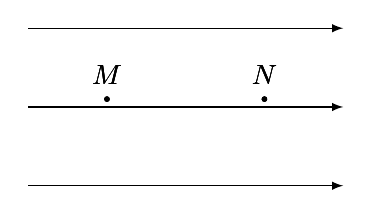
\begin{tikzpicture}[>=latex]
\foreach \x in {1,2,3}
{
    \draw[->] (0, \x)--(4,\x);
\node at (1, 2.4){$M$};  \node at (3, 2.4){$N$};
\fill (1,2.1) circle (1pt); \fill (3,2.1) circle (1pt);
}
        
    \end{tikzpicture}

    \caption{}
\end{figure}	

\item  电子在原子核附近运动时,电子的电势能是正值还
是负值?取无限远处的电势能为零,把这个电子由原子核附
近移到无限远处,电子的电势能是增加还是减小?
\end{enumerate}



\subsection{练习六}

\begin{enumerate}
	\item 电场中A点的电势是3伏,求;
	\begin{enumerate}
		\item 电量为5库的电荷在$A$点的电势能;
		\item 电量为10库的电荷在$A$点的电势能;
		\item 电量为$-5$库的电荷在$A$点的电势能;
		\item 电量为$-10$库的电荷在$A$点的电势能.
	\end{enumerate}
	\item 在图6.16中$A$、$B$两点哪一点电势高?在图6.17中
$C$、$D$两点哪一点的电势高?说明理由.

\item 在图6.23所示的匀强
电场中,如果$A$板是接地的,
$M$、$N$两点哪点电势高?电势是
正值还是负值?如果$B$板是接
地的,结果又怎样?取大地的电
势为零.

\begin{figure}[htp]\centering
    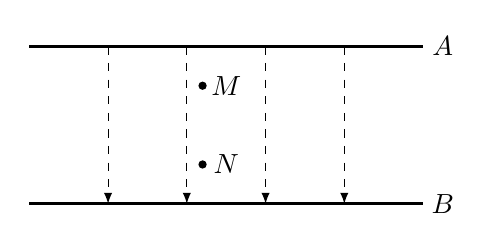
\begin{tikzpicture}[>=latex]
\foreach \x in {0,2}
{
    \draw[very thick] (0,\x) --(5,\x);
}

\node at (5.25,0){$B$};
\node at (5.25,2){$A$};

\foreach \x in {1, 2,3,4}
{
    \draw[->, dashed](\x,2)--(\x,0);
}   
\node at (2.5,1.5){$M$};    \node at (2.5,.5){$N$};
\fill (2.2,1.5) circle (1.5pt);\fill (2.2,.5) circle (1.5pt);
    \end{tikzpicture}
    \caption{}
\end{figure}	

\item 一个初速度为零的正电荷放在电场中,只在电场力
作用下,它向电势高的地方跑还是向电势低的地方跑?一个初
速度为零的电子放在电场中,它向电势高的地方跑还是向电
势低的地方跑?说明理由.
\item 一个初速度为零的电荷放在电场中,不论是正电荷
还是负电荷,都向着电势能低的地方跑,试说明理由.
\item 电场中某点的电势是否跟检验电荷的正负有关?讨
论一下这个问题.
\item 电场中两个电势不同的等势面能不能相交?为什么?
\end{enumerate}



\subsection{练习七}

\begin{enumerate}
	\item 把带电体从电势为300伏的$A$点移到电势为100伏
的$B$点,电场力做了$3.0\x10^{-8}$焦的负功,带电体带哪种电
荷?电量是多少?
\item 电场中$M$、$N$两点的电势$U_M=800$伏、$U_N=-200$
伏,把电量是$1.5\x10^{-8}$库的负电荷从$M$点移到$N$点,电场力
做了多少功?做正功还是负功?
\item 在电场中把电量为$2.0\x10^{-8}$库的正电荷从$A$点移
到$B$点,电场力做了$1.5\x10^{-7}$焦的正功,再把这个正电荷从
$B$点移到$C$点,电场力做了$4.0\x10^{-7}$焦的负功、$A$、$B$、$C$三点
中哪点的电势最高,哪点的电势最低?$A$、$B$间,$B$、$C$间和$A$、$C$
间的电势差各是多大?
\item 一个原来静止的电子,从电场中的$A$点被加速移到
$B$点.$A$、$B$两点间的电势差是2000伏,电场力所做的功是多
少电子伏?电势能的变化是多少电子伏?设电子是在真空中
移动的,电子在$B$点获得的动能是多少电子伏?
\end{enumerate}


\subsection{练习八}

\begin{enumerate}
	\item 两块相距0.05米的带电平行板之间的电场是匀强
	电场,两板的电势差为$10^4$伏.求作用在两板之间的一个电
	子上的电场力.
	\item 平行的带电金属板$A$、$B$间是匀强电场(图6.26),场
	强为$1.2\x10^8\NC$.两板间的距离为5厘米,两板间的电
	势差有多大?电场中有两点$P_1$和$P_2$,$P_1$点离$A$板的距离是
	0.5厘米,$P_2$点离$B$板的距离也是0.5厘米.$P_1$和$P_2$两点间
	的电势差有多大?
\end{enumerate}


\subsection{练习九}
\begin{enumerate}
	\item 在真空中有一对平行金属板,相距6.2厘米,加上90
伏的电压,两价的氧离子从静止出发被加速,从一板到达另
一板时,它的动能是多大?

这道题有几种解法?哪种解法比较简便?

\item 两价离子在90伏的电压下从静止加速后,测出它的
动量是$1.24\x10^{-21}{\rm kg}\cdot \ms$,这种离子的质量是多大?

\item 经1000伏加速电压加速后的电子,沿着与电场垂直
的方向进入匀强偏转电场,场强为5000$\NC$.已知偏转电
极长为6厘米,求电子离开偏转电场时的速度.
\item 计算一下本节例题中的电子离开偏转电场时侧向移
动的距离.
\item 图6.30所示的实验装置可以用来验证电场对带电
粒子的加速作用只跟电压有关.左边的非匀强电场使电子加
速,右边的匀强电场使电子减
速,设非匀强电场的电压为$U$,
匀强电场的电压为$U'$.实验结
果是:只要$U'<U$,电流计的指
针就偏转;只要$U'>U$,电流计
的指针就不偏转.你从这个实
验结果可以得出什么结论?
\begin{figure}[htp]\centering
%	\includegraphics[scale=.6]{fig/6-30.png}
	\caption{}
	\end{figure}
\end{enumerate}



\subsection{练习十}
\begin{enumerate}
	\item 电容器带电后电势差增大的情形,跟物体吸收热量后温度升高的情形也很相似,试对这两种现象作一比较.
	\item 一个由圆板制成的平行板电容器,圆板的半径为3.0
厘米,两板的距离为2.0毫米,中间充满介电常数为6.0的电
介质,这个电容器的电容是多少?
\item 一个电容器的电容是$1.5\x10^{-2}$微法,把它的两个极
板接在90伏的电源上,求每个极板上的电量.
\item 有一个电容器,在带了电量$Q$以后,两导体间的电势
差是$U$,如果使它带的电量增加$4.0\x10^{-8}$库,两导体间的电
势差就增大20伏,这个电容器的电容是多少微法?

\begin{figure}[htp]\centering
    \begin{circuitikz}[european, scale=.8]
        \draw (0,0)--(0,3);
        \draw (0,3)to [capacitor=$C$](6,3);
        \draw (6,0)--(6,3);    
        \draw (0,0) to [battery2] (3,0) to [cute open switch=$K$] (5,0)--(6,0)   ;
    \end{circuitikz}
    \caption{}
\end{figure}

\item 如图6.39所示,闭合
电键$K$使平行板电容器$C$充
电,然后断开电键,当增大电容
器两板间的距离时,下述各量
是否改变,怎样改变?
\begin{enumerate}
	\item 电容器所带电量;
	\item 电容器的电容;
	\item 电容器两板间的电势差.
\end{enumerate}
\item 在上题中,充电后如果保持电键$K$闭合,那么,增大
电容器两板间的距离时,下述各量是否改变,怎样改变?
\begin{enumerate}
	\item 电容器两板间的电势差;
	\item 电容器的电容;
	\item 电容器所带的电量.
\end{enumerate}
\end{enumerate}



\subsection{练习十一}

\begin{enumerate}
\item 两个相同的电容器,标有“100皮法、600伏”,串联后
接到900伏的电路上,每个电容器带多少电?加在每个电容器
上的电压是多少?电容器是否会击穿?
\item 把“100皮法、600伏”和“300皮法、300伏”的电容器
串联后接到900伏的电路上,这样连接是否合适?为什么?
\item 平行板电容器的正对面积为$S$,
两板距离为$\ell$,电介质是真空.如果在两
板之间插入一厚度为$d$的金属板(图6.42),试证明它的电容为
\[C=\frac{S}{4\pi k(\ell-d)}\]
\begin{figure}[htp]\centering
    \begin{tikzpicture}[>=latex]
\draw[ultra thick] (-0.5,0)--(0,0);
\draw[ultra thick] (1,0)--(1.5,0);
\draw [ultra thick] (0,-1.8)--(0,1.8);
\draw[ultra thick]  (1,-1.8)--(1,1.8);
\fill [pattern=north east lines, draw ](.4,-1.8) rectangle (.6,1.8);
\draw (0,-2)--(0,-2.5);\draw (1,-2)--(1,-2.5);
\draw [<->](0,-2.25)--node[fill=white]{$\ell$}(1,-2.25);
\draw (.4,2)--(.4,2.5);\draw (.6,2)--(.6,2.5);
\draw [->](0,2.25)--(.4,2.25);
\draw [->](1,2.25)--(.6,2.25);
\node at (.5,2.5){$d$};
    \end{tikzpicture}

    \caption{}
\end{figure}
\item 电容分别为20微法和50微法的
两个电容器并联后,接在电压为100伏的
电路上,它们共带多少电?
\item 电容为 3000 皮法的电容器带电
$1.8\x10^{-6}$库后,撤去电源,再把它跟电容为1500皮法的电容
器并联,求每个电容器所带电量.
\end{enumerate}





\subsection{习题}
\begin{enumerate}
\item 有一个绝缘的金属筒,上面开个小孔,通过小孔放入
一个悬挂在丝线上的带正电的小球,在下列各种情况里,金
属筒外壁各带什么电荷?
\begin{enumerate}
\item 小球跟筒的内壁不接触;
\item 小球跟筒的内壁接触;
\item 小球跟筒的内壁不接触,但用手指接
触一下金属筒,然后移开手指,再把小球移出筒外.
\end{enumerate}

\item 有两个带电小球,电量分别为$+Q$和$+9Q$,在真空
中相距0.4米.如果引进第三个带电小球,正好使三个小球都
处于平衡状态,第三个小球带的是哪种电荷?应放在什么地
方?电量是$Q$的几倍.
\item 如图6.43所示,有两
个挂在丝线上的小球,带有等
量的同种电荷,由于电荷彼此
推斥,丝线都偏离竖直线$\theta$角,
已知两小球的质量都为$m$,两丝线长都为$\ell$,求每个小球上所带的电量.

\begin{figure}[htp]
\centering
\begin{minipage}[t]{0.48\textwidth}
\centering
\begin{tikzpicture}[scale=.9]
	\draw (0,0)--(2,-5);
	\draw (0,0)--(-2,-5);	
	\draw [dashed](0,0)--(0,-6);
	\draw  (2,-5)[fill=gray] circle (5pt);
	\draw  (-2,-5)[fill=gray] circle (5pt);
	\node at (-1.5, -2.5){$\ell$};	\node at (1.5, -2.5){$\ell$};
	\node at (-2.5, -5){$m$};	\node at (2.5, -5){$m$};
	\draw (0,-1) arc (-90:-112:1) node [below]{$\theta$};
	\draw (0,-.9) arc (-90:-68:.9) node [below]{$\theta$};
\end{tikzpicture}
\caption{}
\end{minipage}
\begin{minipage}[t]{0.48\textwidth}
\centering
    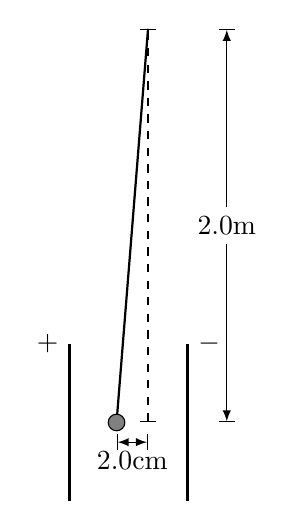
\begin{tikzpicture}[>=latex]
\draw [|<->|](0,0)--node [fill=white]{2.0m}(0,5);
\draw [|-|, dashed](-1,0)--(-1,5);        
\draw [thick](-1.4,0)--(-1,5); 
\draw[fill=gray] (-1.4,0) circle (3pt);

\draw[very thick] (-2, -1)--(-2, 1)node [left]{$+$}; \draw[very thick] (-.5, -1)--(-.5, 1)node [right]{$-$};
\draw [|<->|] (-1.4,-.25)--node [below]{2.0cm}(-1,-.25);


    \end{tikzpicture}
\caption{}
\end{minipage}
\end{figure}



\item 在氢原子中,可以认为核外电子沿圆形轨道绕原子
核(质子)旋转,轨道半径为$5.3\x10^{-11}$米,电子沿轨道运动
的动能是多大?
\item 下面一些说法哪个正确,哪个错误?说明理由.
\begin{enumerate}
\item 在匀强电场中电势处处相等.
\item 沿着电力线的方向场强越来越小.
\item 正电荷在电场中只能由电势高的地方向电势低的地
方跑.
\item 电荷在电场中只能向着电势能低的地方跑.
\item 初速度为零的电荷在电场中一定向着电势能低的地
方跑.
\end{enumerate}
\item 两块靠近的平行金属板,在两板之间为真空时,使它
们分别带上等量的异种电荷,保持两板带的电量不变,如果
将两板间的距离减小为原来的1/3,两板间的电势差是原来
的多少倍?两板间匀强电场的场强是原来的多少倍?
\item 上题中,保持两板带的电量不变,而在两板间充满介
电常数为8的电介质,两板间的电势差和匀强电场的场强将
如何改变?
\item 有一个电容器,电容是$1.5\x10^{-4}$微法,把它的两板
分别跟直流电源的正负极相连,使两板分别带电$6\x10^{-8}$库
和$-6\x10^{-8}$库,如果两板的距离为1毫米,电容器两板间的
电场强度是多大?
\item 两个相当大的平行金属板相
距10厘米,两板分别跟电池组的正
负极连接,两板间的一个小电荷受到
的电场力为$3\x10^{-4}$牛,现在把两板
的距离增加到15厘米,如果连接的电
池组不变,小电荷受到的力变为多大?
如果在增大两板距离时把所连电池组
换成3倍电压的电池组,小电荷受到
的力又将变为多大?



\item 如图 6.44,质量为$4.5\x
10^{-3}$千克的带电小球用2.0米长的线
悬挂在带等量异种电荷的平行板之
间,平衡时小球偏离竖直位置 2.0厘
米.
\begin{enumerate}
	\item 小球受到的电场力是多大?
	\item 如果两板间的电压是$1.5\x10^4$伏,两板的距离是10厘米,
那么,小球带有多少个多余的电子?
\end{enumerate}
	

\item 在图6.29中,先让一束电子,后让一束氢核通过偏
转电场,设电子和氢核的初速度相同,电子和氢核原来
的动能相同,试分别求出两种情况下电子的偏角$\phi_e$和氢核
的偏角$\phi_H$的正切之比.

\begin{figure}[htp]\centering
%	\includegraphics[scale=.5]{fig/6-45.png}
	\caption{}
	\end{figure}
	
\item 图6.45是用来使带正电的粒子加速和偏转的装
置,如果让氢和氦进入并电离,我们将得到一价氢离子,一价
氦离子和二价氦离子的混合物.它们经过同一电场加速后,
在同一电场里偏转,它们是否会分为三股,从而到达荧光屏后
产生三个亮点?回答中要说明理由.

\end{enumerate}

















